% This LaTeX was auto-generated from MATLAB code.
% To make changes, update the MATLAB code and export to LaTeX again.

\documentclass{article}

\usepackage[utf8]{inputenc}
\usepackage[T1]{fontenc}
\usepackage{lmodern}
\usepackage{graphicx}
\usepackage{color}
\usepackage{hyperref}
\usepackage{amsmath}
\usepackage{amsfonts}
\usepackage{epstopdf}
\usepackage[table]{xcolor}
\usepackage{matlab}
\usepackage[paperheight=795pt,paperwidth=614pt,top=72pt,bottom=72pt,right=72pt,left=72pt,heightrounded]{geometry}

\sloppy
\epstopdfsetup{outdir=./}
\graphicspath{ {./hw8_media/} }

\begin{document}


\title{Homework 8: Statistical Estimation, Numerical Methods for Eigenvalues, and SVD}
\author{Matthew Luyten\\
ECE6250}

\maketitle

\matlabheading{Problem 8.1}

\vspace{1em}
\begin{par}
\begin{flushleft}
This week, we learned different forms of matrix decomposition, which is an important part of statistical estimation. In ECE6001, we are 
currently studying MSE-minimizing linear predictors using cholesky decomposition. This is interestingly similar
to the BLUE method we covered, and a way to handle prediciton as oposed to the estimation we have covered.
\end{flushleft}
\end{par}

\begin{par}
\begin{flushleft}
First, we covered the power method for finding eigenvalues, which was an interesting brute-force approach. It's very
simple, so it is easy to implement; however, it can become very computationally intensive if the difference
between the largest eigenvalue and the second-largest eigenvalue is small. We also learned about singular value
decomposition. This gives us an elegant way to break down an uninvertible matrix and find a solution to the
linear inverse problem. 
\end{flushleft}
\end{par}

\begin{par}
\begin{flushleft}
We also covered the pseudo-inverse, which is an important tool as many real-world problems cannot be simplified to an
invertible matrix. The pseudo-inverse gives us a tool to use when an inverse is impossible, and under the right
circumstances, it can provide a solution that minimizes MSE.
\end{flushleft}
\end{par}


\newpage
\matlabheading{Problem 8.2}

\begin{par}
\begin{flushleft}
\textit{Part B} - Find $\mathit{\mathbf{x}}$ such that $\textrm{Ax}=\left\lbrack \begin{array}{c}
1\\
1
\end{array}\right\rbrack$
\end{flushleft}
\end{par}

\begin{par}
\begin{flushleft}
$\mathit{\mathbf{x}}={\mathit{\mathbf{A}}}^{-1} \mathit{\mathbf{y}}$, $\mathit{\mathbf{x}}=\left\lbrack \begin{array}{c}
-1\ldotp 0204\\
2\ldotp 0408
\end{array}\right\rbrack$
\end{flushleft}
\end{par}

\begin{matlabcode}
A = [[1.02 1]; [1 0.99]];
y = [1; 1];
x = A\y;
display(x);
\end{matlabcode}
\begin{matlaboutput}
x = 2x1    
   -1.0204
    2.0408

\end{matlaboutput}


\begin{par}
\begin{flushleft}
\textit{Part C} - Find $\mathit{\mathbf{x}}$ such that $\mathit{\mathbf{Ax}}=\left\lbrack \begin{array}{c}
1\ldotp 1\\
1
\end{array}\right\rbrack$
\end{flushleft}
\end{par}

\begin{par}
\begin{flushleft}
A small perturbation in $\mathit{\mathbf{y}}$ caused a large perturbation in $\mathit{\mathbf{x}}$! $||{\mathit{\mathbf{y}}}_1 -{\mathit{\mathbf{y}}}_2 ||_2^2 =0\ldotp 01$, $||{\mathit{\mathbf{x}}}_1 -{\mathit{\mathbf{x}}}_2 ||_2^2 =206\ldotp 1745$
\end{flushleft}
\end{par}

\begin{matlabcode}
A = [[1.02 1]; [1 0.99]];

y1 = [1; 1];
x1 = A\y1;

y2 = [1.1; 1];
x2 = A\y2;

display(x1);
\end{matlabcode}
\begin{matlaboutput}
x1 = 2x1    
   -1.0204
    2.0408

\end{matlaboutput}
\begin{matlabcode}
display(x2);
\end{matlabcode}
\begin{matlaboutput}
x2 = 2x1    
    9.0816
   -8.1633

\end{matlaboutput}
\begin{matlabcode}
fprintf("Norm Squared Error in y: %f", norm(y1-y2)^2);
\end{matlabcode}
\begin{matlaboutput}
Norm Squared Error in y: 0.010000
\end{matlaboutput}
\begin{matlabcode}
fprintf("Norm Squared Error in x: %f", norm(x1-x2)^2);
\end{matlabcode}
\begin{matlaboutput}
Norm Squared Error in x: 206.174511
\end{matlaboutput}



\vspace{1em}
\begin{par}
\begin{flushleft}
\textit{Part D} - Find the unit vector ${\mathit{\mathbf{e}}}_{\max }$ which maximizes $||\tilde{\mathit{\mathbf{x}}} -\mathit{\mathbf{x}}||_2^2$
\end{flushleft}
\end{par}

\begin{par}
\begin{flushleft}
We know that the unit eigenvector corresponding with the largest eigenvalue will yield the maximum error, so ${\mathit{\mathbf{e}}}_{\max } =\left\lbrack \begin{array}{c}
0\ldotp 7124\\
0\ldotp 7018
\end{array}\right\rbrack$
\end{flushleft}
\end{par}


\begin{par}
\begin{flushleft}
\textit{Part E} - Find the unit vector $e_{\min }$ which maximizes $||\tilde{\mathit{\mathbf{x}}} -\mathit{\mathbf{x}}||_2^2$
\end{flushleft}
\end{par}

\begin{par}
\begin{flushleft}
We know that the unit eigenvector corresponding with the smallest eigenvalue will yield the maximum error, so ${\mathit{\mathbf{e}}}_{\max } =\left\lbrack \begin{array}{c}
-0\ldotp 7018\\
0\ldotp 7124
\end{array}\right\rbrack$
\end{flushleft}
\end{par}


\begin{par}
\begin{flushleft}
\textit{Part F} - What is the mean-square error $\mathrm{E}\left\lbrack ||\tilde{\mathit{\mathbf{x}}} -\mathit{\mathbf{x}}||_2^2 \right\rbrack$
\end{flushleft}
\end{par}

\begin{par}
\begin{flushleft}
$\mathrm{E}\left\lbrack ||\tilde{\mathit{\mathbf{x}}} -\mathit{\mathbf{x}}||_2^2 \right\rbrack =\mathrm{E}\left\lbrack ||{\mathit{\mathbf{A}}}^{-1} \mathit{\mathbf{e}}||_2^2 \right\rbrack$ and we know that $E\left\lbrack ||{\mathit{\mathbf{A}}}^{-1} \mathit{\mathbf{e}}||_2^2 \right\rbrack =\sigma^2 \sum_{n=1}^N \frac{1}{\lambda_n^2 }$, so $\mathrm{E}\left\lbrack ||\tilde{\mathit{\mathbf{x}}} -\mathit{\mathbf{x}}||_2^2 \right\rbrack =41816.3$
\end{flushleft}
\end{par}


\begin{par}
\begin{flushleft}
P\textit{art G} - Confirm the solution to \textit{F} with 10,000 realizations of e
\end{flushleft}
\end{par}

\begin{par}
\begin{flushleft}
The average error is close to 41816.3. See below.
\end{flushleft}
\end{par}

\begin{matlabcode}
A = [[1.02 1]; [1 0.99]];
y = [1; 1];
x = A\y;

error = 0;
for i = 1:10000
    x_hat = A\(y-randn(2,1));
    error = error + norm(x-x_hat)^2;
end

fprintf("Avg Error: %f", error / 10000);
\end{matlabcode}
\begin{matlaboutput}
Avg Error: 42039.287865
\end{matlaboutput}

\newpage
\matlabheading{Problem 8.3}

\begin{par}
\begin{flushleft}
\textit{Part A }- Write a matlab function that uses the power iteration procedure to find the largest eigenvalue of matrix A and its associated eigenvalue
\end{flushleft}
\end{par}

\begin{matlabcode}
function [lambda, v, it] = pm_eig(A)
    sz = size(A);
    sz(2) = 1;
    
    z = ones(sz);
    q = z / norm(z);
    q_prev = zeros(sz);
    it = 0;
    while norm(q-q_prev) > eps && norm(q-q_prev) < 2.0 - eps
        q_prev = q;
        z = A*q_prev;
        q = z / norm(z);
        it = it + 1;
        norm(q-q_prev);
        if it > 1e5
            break
        end
    end
    
    v = q;
    lambda = q.'*A*q;
end
\end{matlabcode}


\begin{matlabcode}
sizes = [10, 100, 1000];

for idx = 1:3
    B = randn([sizes(idx), sizes(idx)]);
    A = B + B.';
    [l, v, i] = pm_eig(A);
    eigs = eig(A);
    eigs = [eigs(1), eigs(end)];
    [~, x] = max(abs(eigs));
    fprintf("%i x %i Matrix", sizes(idx), sizes(idx));
    fprintf("\tMax Eigenvalue (Power Method): %f", l);
    fprintf("\tMax Eigenvalue (Matlab eig): %f", eigs(x));
    fprintf("\tIterations %i\n", i);
end
\end{matlabcode}
\begin{matlaboutput}
10 x 10 Matrix
	Max Eigenvalue (Power Method): -8.132805
	Max Eigenvalue (Matlab eig): -8.132805
	Iterations 421
100 x 100 Matrix
	Max Eigenvalue (Power Method): -28.302064
	Max Eigenvalue (Matlab eig): -28.302064
	Iterations 1729
1000 x 1000 Matrix
	Max Eigenvalue (Power Method): -89.482975
	Max Eigenvalue (Matlab eig): -89.482975
	Iterations 2207
\end{matlaboutput}


\begin{par}
\begin{flushleft}
\textit{Part C} - The number of iterations increases as the matrix size increases. This makes sense, as the power method requires more iterations to converge when the largest and second-largest eigenvalues are close in value. The larger a matrix becomes, the more eigenvalues it has, so there are more opportunities to for $|\lambda_1 |$ and $|\lambda_2 |$ be similar values.
\end{flushleft}
\end{par}

\begin{par}
\begin{flushleft}
\textit{Part B - }My code and matlab's eig function return the same largest eigenvalues. See a sample output from the above code:
\end{flushleft}
\end{par}

\begin{par}
\begin{flushleft}
\texttt{10 x 10 Matrix}
\end{flushleft}
\end{par}

\begin{par}
\begin{flushleft}
\texttt{	Max Eigenvalue (Power Method): 8.839135}
\end{flushleft}
\end{par}

\begin{par}
\begin{flushleft}
\texttt{	Max Eigenvalue (Matlab eig): 8.839135}
\end{flushleft}
\end{par}

\begin{par}
\begin{flushleft}
\texttt{	Iterations 283}
\end{flushleft}
\end{par}

\begin{par}
\begin{flushleft}
\texttt{100 x 100 Matrix}
\end{flushleft}
\end{par}

\begin{par}
\begin{flushleft}
\texttt{	Max Eigenvalue (Power Method): -27.034852}
\end{flushleft}
\end{par}

\begin{par}
\begin{flushleft}
\texttt{	Max Eigenvalue (Matlab eig): -27.034852}
\end{flushleft}
\end{par}

\begin{par}
\begin{flushleft}
\texttt{	Iterations 983}
\end{flushleft}
\end{par}

\begin{par}
\begin{flushleft}
\texttt{1000 x 1000 Matrix}
\end{flushleft}
\end{par}

\begin{par}
\begin{flushleft}
\texttt{	Max Eigenvalue (Power Method): -89.070349}
\end{flushleft}
\end{par}

\begin{par}
\begin{flushleft}
\texttt{	Max Eigenvalue (Matlab eig): -89.070349}
\end{flushleft}
\end{par}

\begin{par}
\begin{flushleft}
\texttt{	Iterations 2198}
\end{flushleft}
\end{par}

\newpage
\matlabheading{Problem 8.4}

\begin{matlabcode}
function y = svd_reconstruct(x, r)
    [U, S, V] = svd(x);
    y = U(:,1:r)*S(1:r,1:r)*V(:,1:r).';
end
\end{matlabcode}


\begin{par}
\begin{flushleft}
\textit{Part A} - Dispay ${\mathit{\mathbf{A}}}_{\mathit{\mathbf{s}}}$ for $s=\left\lbrack 500,200,100,30,10\right\rbrack$
\end{flushleft}
\end{par}

\begin{matlabcode}
A = double(imread("flower.png"));
A0 = svd_reconstruct(A, 50);

image(A); 
colormap("gray"); 
axis square;
axis off; 
title("A_s (s = 500)");
\end{matlabcode}
\begin{center}
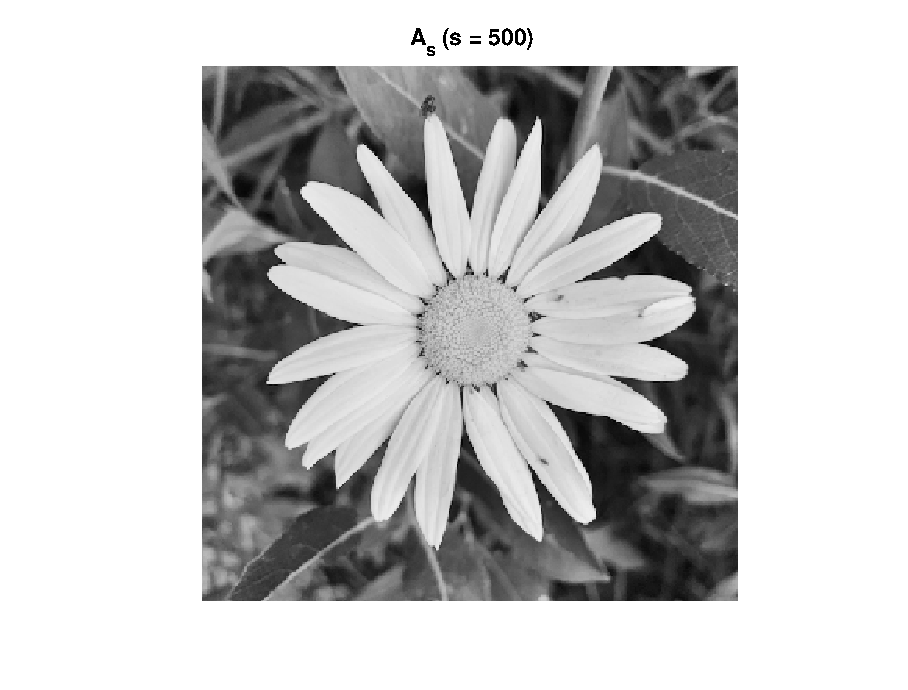
\includegraphics[width=\maxwidth{56.196688409433015em}]{figure_0.eps}
\end{center}
\begin{matlabcode}

image(uint8(svd_reconstruct(A, 200))); 
colormap("gray"); 
axis square;
axis off;
title("A_s (s = 200)");
\end{matlabcode}
\begin{center}
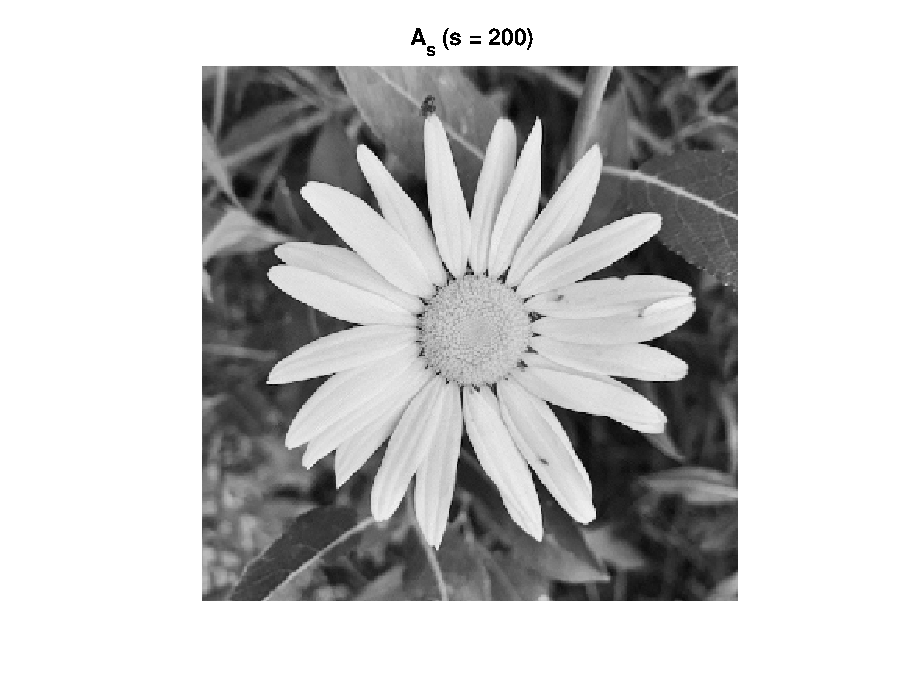
\includegraphics[width=\maxwidth{56.196688409433015em}]{figure_1.eps}
\end{center}
\begin{matlabcode}

image(uint8(svd_reconstruct(A, 100))); 
colormap("gray"); 
axis square;
axis off;
title("A_s (s = 100)");
\end{matlabcode}
\begin{center}
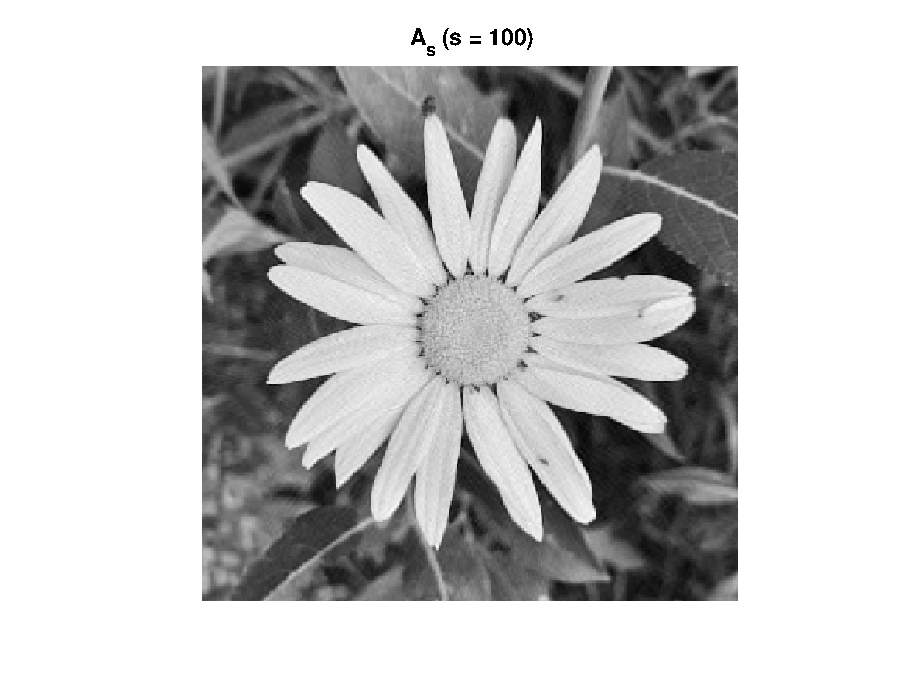
\includegraphics[width=\maxwidth{56.196688409433015em}]{figure_2.eps}
\end{center}
\begin{matlabcode}

image(uint8(svd_reconstruct(A, 30))); 
colormap("gray"); 
axis square;
axis off;
title("A_s (s = 30)");
\end{matlabcode}
\begin{center}
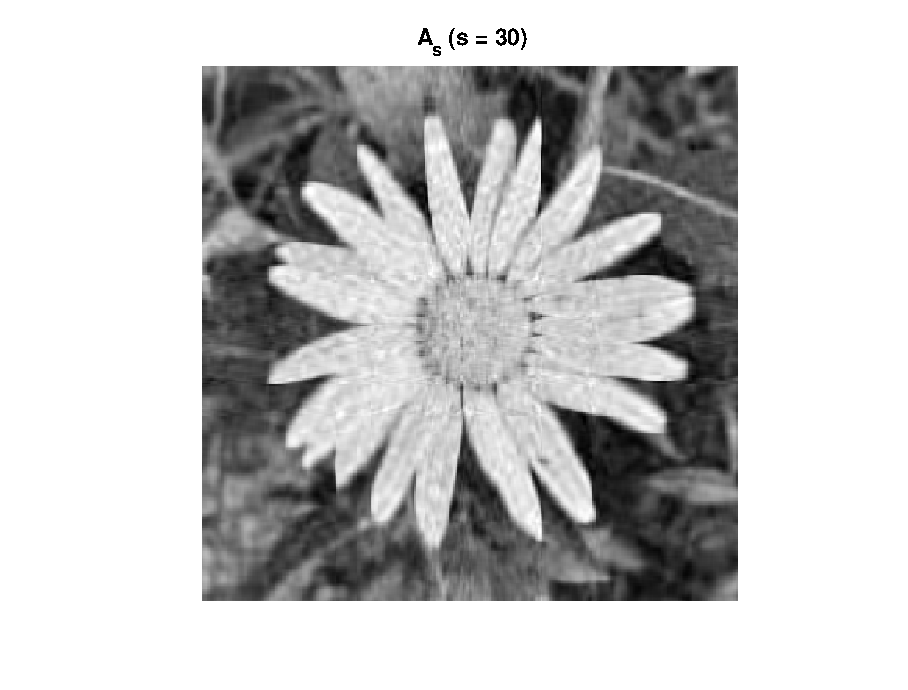
\includegraphics[width=\maxwidth{56.196688409433015em}]{figure_3.eps}
\end{center}
\begin{matlabcode}

image(uint8(svd_reconstruct(A, 10))); 
colormap("gray"); 
axis square;
axis off;
title("A_s (s = 10)");
\end{matlabcode}
\begin{center}
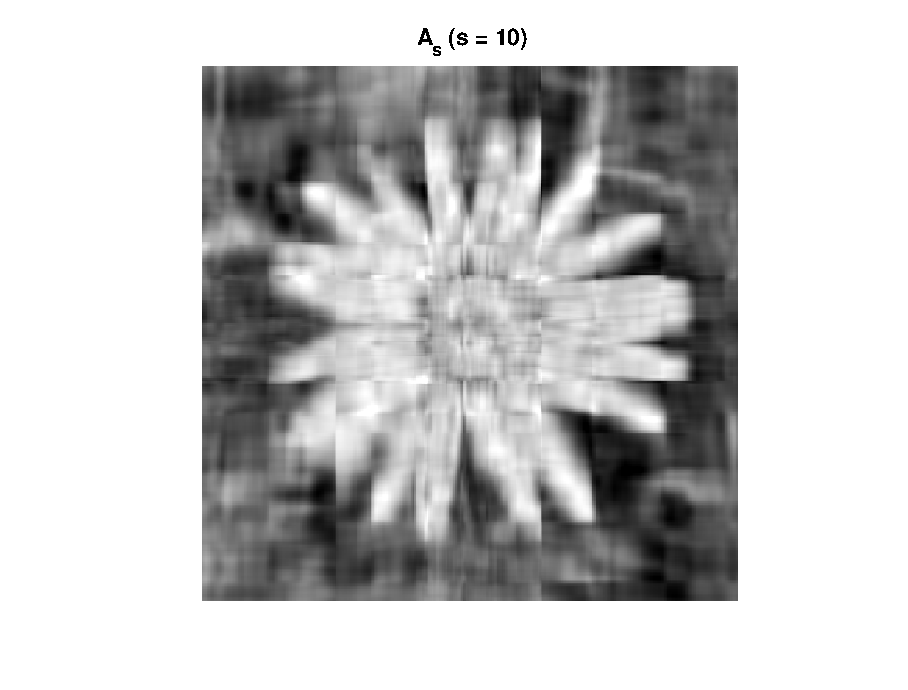
\includegraphics[width=\maxwidth{56.196688409433015em}]{figure_4.eps}
\end{center}


\begin{par}
\begin{flushleft}
\textit{Part B} - How many values are required to represent ${\mathit{\mathbf{A}}}_{\mathit{\mathbf{s}}}$ when $s\not= 500$?
\end{flushleft}
\end{par}

\begin{par}
\begin{flushleft}
${\mathit{\mathbf{u}}}_{s\;} \in {\mathbb{R}}^{500\;x\;S}$, ${\mathit{\mathbf{v}}}_s^T \in {\mathbb{R}}^{S\;x\;500}$, and $\sigma_s$\textbf{ }has $s$ non-zero values, therefore, the SVD representation with $s$ singular values has $2\left(500\times s\right)+s$ values.
\end{flushleft}
\end{par}

\begin{matlabcode}
s = [200, 100, 30, 10];

for idx = 1:4
    vals = 500 * s(idx) * 2 + s(idx);
    fprintf("Number of values to represent A with %i sv's: %i\n", s(idx), vals);
end
\end{matlabcode}
\begin{matlaboutput}
Number of values to represent A with 200 sv's: 200200
Number of values to represent A with 100 sv's: 100100
Number of values to represent A with 30 sv's: 30030
Number of values to represent A with 10 sv's: 10010
\end{matlaboutput}

\end{document}
